\documentclass{beamer-control}
\usepackage{beamer-control-singlefile}
\INCLUDEONLY{Integral Action}
\begin{document}
\CONCEPT{Integral Action}

\begin{SUMMARY}
\begin{itemize}
\item System augmentation
\item Reachability of the augmented system
\end{itemize}
\vfill References:
\begin{itemize}
\item \astrom{§7.4}
\end{itemize}
\end{SUMMARY}



\SUBCONCEPT{System augmentation}

\begin{frame}{Integral action}
\begin{itemize}
\item When a perfect model is available, state feedback allows systems in closed-loop to track command signals
\item In cases where our model is only approximately accurate, our controller may have non-zero steady-state error
\item It may be beneficial then, to use integral feedback by feeding back the integral of the error signal
\item When integral feedback is applied, even if we have errors in our model parameters or disturbances to our system, the controller will compensate and result in perfect tracking
\end{itemize}
\end{frame}

\begin{frame}{Integral action}
The idea is to add an additional state to our system that computes the integral of the error signal which is then fedback into the input. We do this by augmenting the system with a new state $z$ which is the integral of the error between the output $y$ and the desired output $r$
\[\frac{\mathrm{d}}{\mathrm{d} t} \begin{bmatrix}
	x \\ z
\end{bmatrix} = 
\begin{bmatrix}
	Ax+Bu\\ y-r
\end{bmatrix} = \begin{bmatrix}
Ax+Bu\\ Cx-r
\end{bmatrix}.\]
To stabilise this system we require $\dot{z}=0$ and therefore $y=r$  (the output matches the desired output).\\
The state space controller for this system is therefore dependent on the state $x$, augmented state $z$ and desired output $r$,
\[u=-Kx-k_iz+k_fr.\]
\end{frame}

\begin{frame}{Example}
The linearised dynamics around an equilibrium point $v_e$, $u_e$, of a cruise control system are 
\[\frac{\mathrm{d}x}{\mathrm{d} t} = -ax-b_g\theta +bw, \quad y=v=x+v_e.\]
The system may be augmented with an integrator to become
\[\frac{\mathrm{d}}{\mathrm{d}t} \begin{bmatrix}
	x \\ z
\end{bmatrix} = \begin{bmatrix}
-a & 0 \\ 1 & 0
\end{bmatrix}  \begin{bmatrix}
x \\ z
\end{bmatrix} +  \begin{bmatrix}
b \\ 0
\end{bmatrix} w +  \begin{bmatrix}
-b_g\\ 0
\end{bmatrix} \theta +  \begin{bmatrix}
0 \\ v_e-v_r
\end{bmatrix}\]
in state space.\\
The constants $a$, $b$, $b_g$ depend on properties of the system, $x=v-v_e$ is the speed around the equilibrium, $w=u-u_e$ is the throttle around the equilibrium , and $\theta$ is the angle of the road.
\end{frame}

\begin{frame}{Example continued}
The controller will be of the form 
\[\frac{\mathrm{d}z}{\mathrm{d}t} = y-v_r, \quad w=-k_px-k_iz+k_fv_r\]
where $v_r$ is the desired reference speed.\\
If we wish to design the closed-loop system to have the desired characteristic polynomial
\[p(s)=s^2+a_1s+a_2\]
then we must compare with the characteristic polynomial of 
\[\operatorname{det}(sI-A+BK) = s^2+(bk_p+a)s+bk_i.\]
Therefore, 
\[k_p=\frac{a_1-a}{b}, \quad k_i=\frac{a_2}{b}, \quad k_f=\frac{a_1}{a}.\]
\end{frame}

\begin{frame}{Example continued}
The figure below shows an example of the cruise control system with reference speed of $20$m/s when the car encounters a hill of $\theta=4^\circ$ at $t=5$s. Both controllers are affected by this disturbance, but the controller with integral action included eventually converges to the desired speed.
\begin{figure}
	\centering
	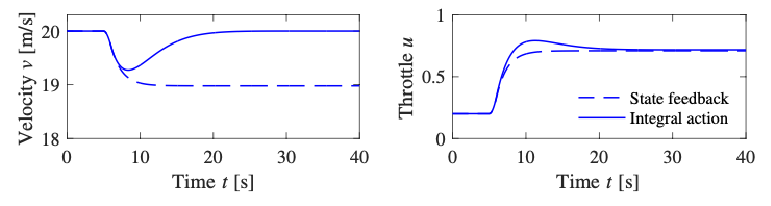
\includegraphics[width=\linewidth]{figure7.12}
	\\
	\textbf{Figure 7.12:} Velocity and throttle for a car with cruise control based on state feedback (dashed) and state feedback with integral action (solid).
\end{figure}
\end{frame}

\SUBCONCEPT{Reachability of the augmented system}

\begin{frame}{Reachability}
\begin{itemize}
\item As we have seen, eigenvalue assignment requires a system to be reachable
\item The reachability matrix for the augmented system is
\[W_r = \begin{bmatrix}
	B & AB & \cdots & A^n B \\
	0 & CB & \cdots & CA^{n-1}B
\end{bmatrix}\]
\item The condition of reachability for the augmented system is equivalent to the condition that $b_n\neq 0$ (the original system does not contain a pure derivative term in the input/output response)
\item In the previous example we see that if $b=0$, there are no values of $k_i$ that make the constant term of our characteristic polynomial equal to the constant term of the desired characteristic polynomial $a_2$
\end{itemize}
\end{frame}


\SUMMARYFRAME
\FINALE

\end{document}
